\chapter{Introduction}
	\section{Are you interested?}
This book is written by a non-specialist of ArchLinux with basic knowledge of 
linux system so I will try to made it as simple as possible for people 
who have no idea about what is console. Indeed, all commands will be 
explained for a better comprehension and an index will be available for you.
\\\\
No matter if you are an expert or a novice, you will be able to find 
how to install stuff on your your Pi plus tips which includes all the problems 
I encounter during my first installation.

	\section{What is a Raspberry Pi}
If you succeed to find this book I guess you allready know but some people 
buy a Raspberry with OpenELEC\footnote{Tiny linux system based on XBMC media center. 
More details on \href{http://openelec.tv}{openelec.tv}} pre-installed so here 
is a little explaination.
\\\\
The Raspberry Pi is a credit-size computer with low performances if you
compare with a common PC. Nevertheless, it means its power consumption is
very low (1W for B+ version\footnote{Most robust version of RPi with 512MB 
of RAM and 4 usb ports}) so it is not a problem to let it on forever. 
\newpage
\begin{figure}[h]
	\centering
	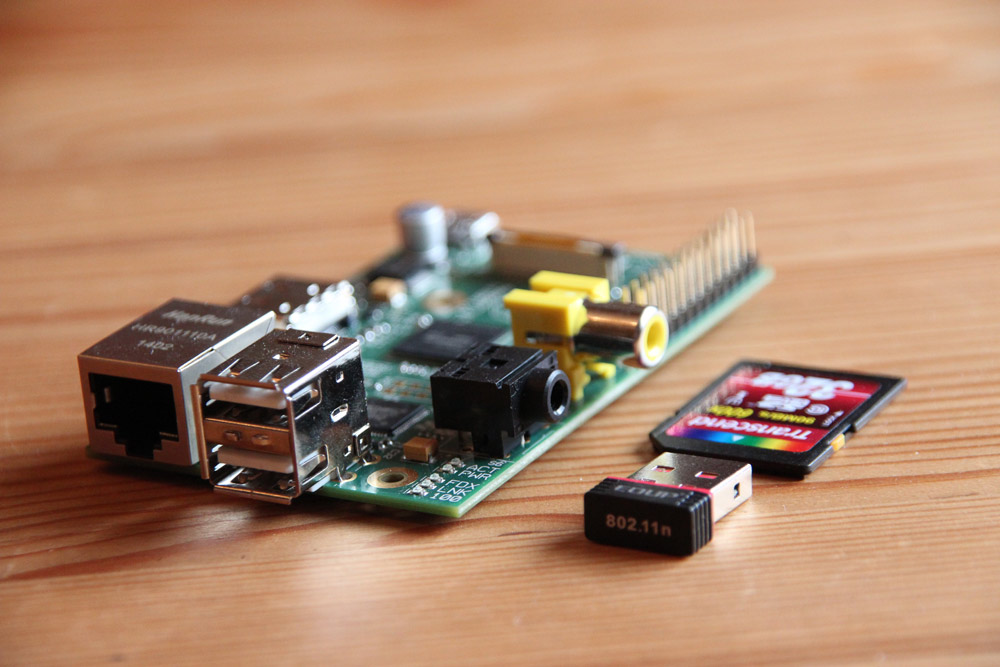
\includegraphics[scale=0.2]{images/RaspberrySize.jpg}
	\caption{Raspberry Pi B+}
	\label{figure:RaspberrySize}
\end{figure}

Finally if you install a good linux distribution on it you can turn this old computer
into a cheap server on which you will have the control. You can use it 
at home for file sharing, media player or others but it is also possible
to host a website which will be available on the internet\footnote{An example
of website hosted by a Rpi on \href{http://raspberrypi.goddess-gate.com}
{raspberrypi.goddess-gate.com}}.

	\section{ArchLinux versus \href{http://www.raspbian.org}{Raspbian}}
	\label{section:ArchVsRaspbian}
The operating system recommended by the Raspberry fundation is Raspbian -- a custom version of the famous Debian\footnote{One of the most popular linux 
system. See \href{https://www.debian.org/intro/about}{debian.org} for more details} system -- optimized for RPi hardware. 
\\\\
In general it will be the default choice for an inexperienced user to get
a user interface and most common softwares allready installed at the first boot.
However we forget the limited performances of the Raspberry and you will be able to realize that for yourself if you decided to install Raspbian. 
\\\\
A server does not need a user interface except a terminal which is enough 
to manage it everyday from anywhere. As a result, my choice has been focused 
on ArchLinux which is a pretty light and fast system. In addition, system 
updates are based on rolling release \footnote{Definition on \href{http://
en.wikipedia.org/wiki/Rolling\_release}{wikipedia/Rolling\_release}} model, 
so it means you do not have one version of the system. You will just receive 
updates frequentely -- as soon as their availability -- and it will be not 
necessary to reboot during the upgrade process.
